% Owner: Keito
\subsubsection{Overview window}
\label{sec:vis-overview}
The overview at the top of the centre column shows the whole recording at once
(Figure~\ref{fig:vis-overview}). It is drawn from at most 4000 points, each with the
minimum and maximum of the samples it stands for, so short peaks remain visible even in
a recording of several hours. Before the \SI{1}{\kilo\hertz} summary is ready the strip
shows the approximate preview (Section~\ref{sec:vis-loading}). After detection, a marker
shows the time of every piece.

A frame on the overview marks the \emph{viewing window}, the time range shown in the
detail window (Section~\ref{sec:vis-detail}). The user can drag the inside of the frame
to move it, drag either side to change its width, or press outside the frame to centre
it there. A slider below the strip sets the width directly (in steps of
\SI{0.1}{\second}) and keeps the centre. The window is at least \SI{0.5}{\second} wide
and at most the whole recording; a new recording opens with the first \SI{5}{\second}.
We wanted one frame that is both moved and resized by dragging, so the strip is a small
custom component drawn on a canvas, which sends the new start and
end to Python when the mouse button is released.

The viewing window is stored once, in \texttt{state.py}, and every control changes it
through the same function: dragging the frame, the width slider, the zoom and pan
buttons of the detail window, a click on the heatmap (Section~\ref{sec:vis-heatmap}) and
the selection of a piece (Section~\ref{sec:vis-events}). This function orders the two
ends, keeps them inside the recording and enforces the minimum width
(\texttt{viewport.py}), so all views always show the same range. Because Streamlit draws
the page from top to bottom on every run, a change that comes from a control below the
slider (for example the heatmap) is applied in a callback before the page is drawn
again, so the slider and the frame always agree.

\begin{figure}[H]
  \centering
  \setlength{\fboxsep}{0pt}%
  \fbox{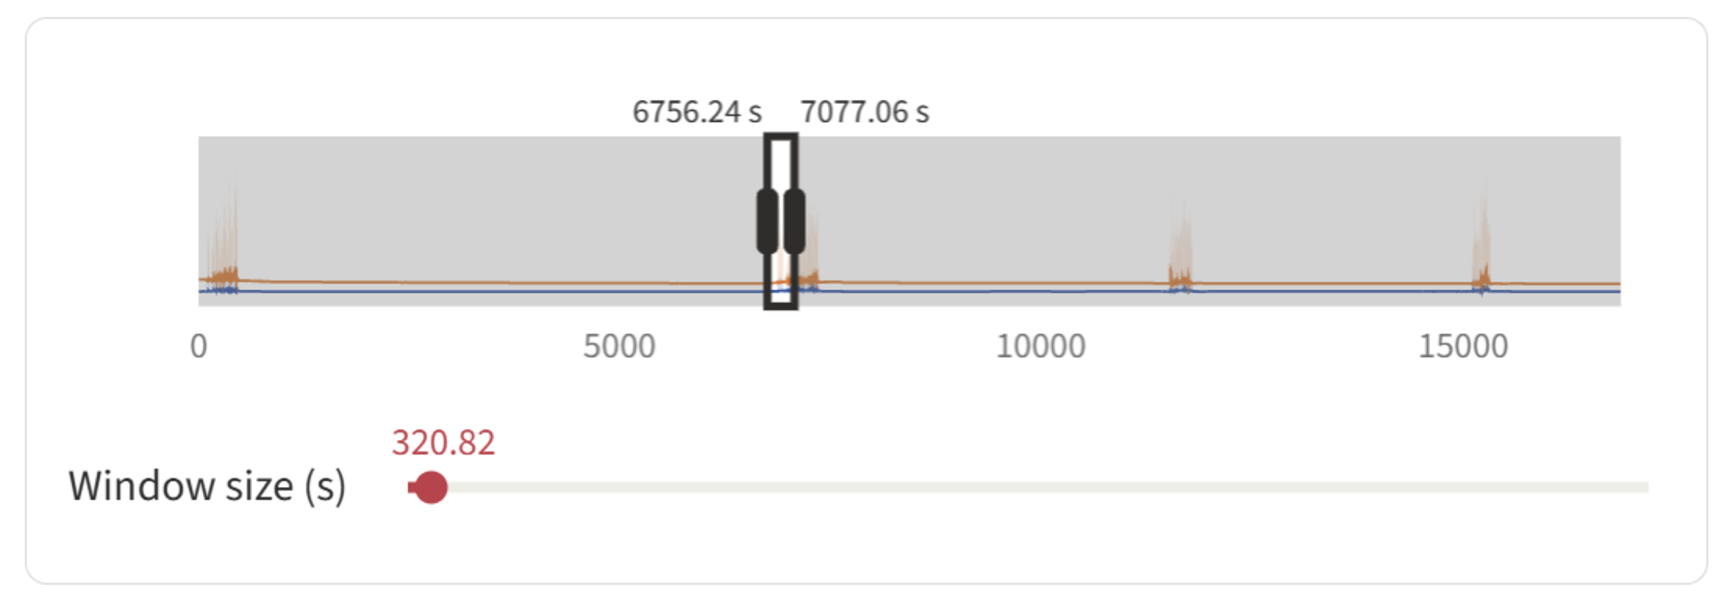
\includegraphics[width=0.8\linewidth]{img/overview.pdf}}
  \caption{Overview strip of a recording of about 4.7\,h. The frame marks the viewing
           window (here \SIrange{6756}{7077}{\second}); its sides are dragged to change
           the width, which is also set with the slider below.}
  \label{fig:vis-overview}
\end{figure}
